% !TeX program = pdflatex
\documentclass[border=6pt]{standalone}
\usepackage{tikz}
\usepackage{amsmath}
\usetikzlibrary{arrows.meta, positioning, calc}

\definecolor{MediumRed}{rgb}{0.925, 0.345, 0.345}
\definecolor{MediumGreen}{rgb}{0.37, 0.7, 0.66}
\definecolor{MediumBlue}{rgb}{0.015, 0.315, 0.45}
\definecolor{DarkBlue}{rgb}{0.05, 0.15, 0.35}

\begin{document}
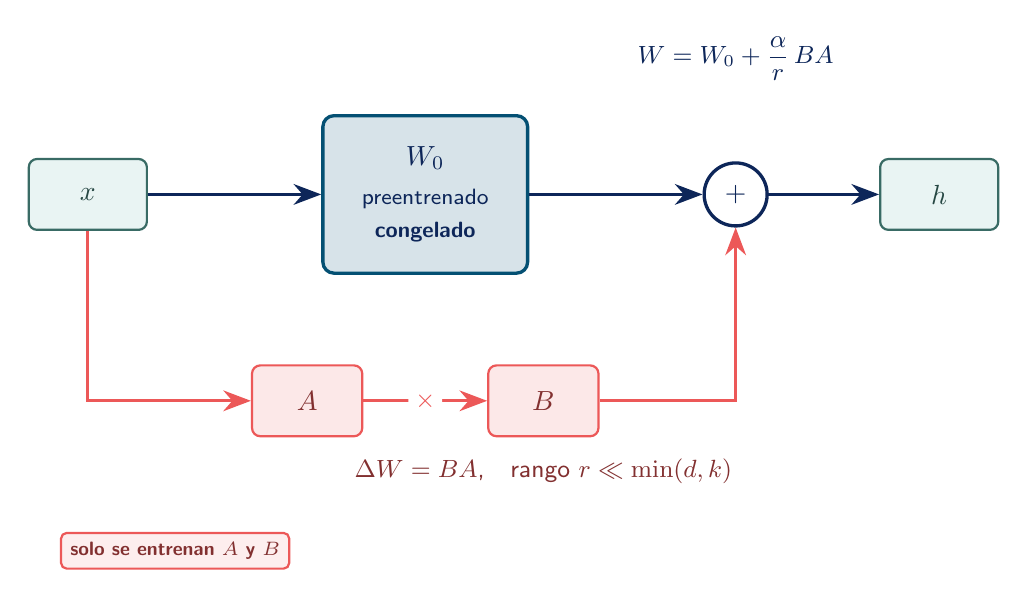
\begin{tikzpicture}[
    font=\sffamily,
    flow/.style={-{Stealth[length=3.5mm]}, line width=1.2pt, DarkBlue},
    io/.style={draw=MediumGreen!60!black, thick, rounded corners=3pt, fill=MediumGreen!14,
        text=MediumGreen!40!black, align=center, minimum width=1.5cm, minimum height=0.9cm},
]

\node[io] (x) at (0,0) {$x$};

% W0 congelado (grande)
\node[draw=MediumBlue, very thick, rounded corners=4pt, fill=MediumBlue!16,
      text=DarkBlue, align=center, minimum width=2.6cm, minimum height=2.0cm,
      right=2.2cm of x] (w0) {$W_0$\\[2pt]\footnotesize preentrenado\\\footnotesize \textbf{congelado}};

% rama LoRA: A luego B (rango bajo)
\node[draw=MediumRed, thick, rounded corners=3pt, fill=MediumRed!14,
      text=MediumRed!55!black, align=center, minimum width=1.4cm, minimum height=0.9cm]
      at ($(w0.south)+(-1.5,-1.6)$) (A) {$A$};
\node[draw=MediumRed, thick, rounded corners=3pt, fill=MediumRed!14,
      text=MediumRed!55!black, align=center, minimum width=1.4cm, minimum height=0.9cm]
      at ($(w0.south)+(1.5,-1.6)$) (B) {$B$};

% suma
\node[draw=DarkBlue, very thick, circle, fill=white, text=DarkBlue,
      minimum size=0.8cm, inner sep=0pt, right=2.2cm of w0] (sum) {$+$};
\node[io, right=1.4cm of sum] (out) {$h$};

% conexiones
\draw[flow] (x) -- (w0);
\draw[flow] (w0) -- (sum);
\draw[flow, MediumRed] (x.south) |- (A);
\draw[flow, MediumRed] (A) -- node[circle, fill=white, inner sep=1pt, font=\sffamily\small] {$\times$} (B);
\draw[flow, MediumRed] (B) -| (sum);
\draw[flow] (sum) -- (out);

% etiquetas
\node[font=\sffamily\small, text=MediumRed!55!black, below=0.15cm of B]
    {$\Delta W = BA$,\quad rango $r \ll \min(d,k)$};
\node[font=\sffamily\small\bfseries, text=DarkBlue, above=0.9cm of sum, align=center]
    {$W = W_0 + \dfrac{\alpha}{r}\,BA$};
\node[draw=MediumRed, thick, rounded corners=2pt, fill=MediumRed!10,
      text=MediumRed!55!black, font=\sffamily\scriptsize\bfseries, below left=1.2cm and -0.5cm of A]
    {solo se entrenan $A$ y $B$};

\end{tikzpicture}
\end{document}
